\documentclass[10pt, journal,letterpaper]{IEEEtran}

\usepackage{color}
\usepackage[american]{babel}
\usepackage{times}
\usepackage{textcomp}

%\usepackage[utf8x]{inputenc}

% 
% Page numbering
% 

% \makeatletter
% \def\ps@headings{
% \def\@oddhead{\mbox{}\scriptsize\rightmark \hfil \thepage}
% \def\@evenhead{\scriptsize\thepage \hfil \leftmark\mbox{}}
% \def\@oddfoot{}
% \def\@evenfoot{}}
% \makeatother
% \pagestyle{headings}


\usepackage{cite,comment,subfigure}

% related to subfigure
\subfigcapmargin = .1cm


% *** GRAPHICS RELATED PACKAGES ***
%
\ifCLASSINFOpdf
  \usepackage[pdftex]{graphicx}
  % declare the path(s) where your graphic files are
  \graphicspath{{./}}
  % and their extensions so you won't have to specify these with
  % every instance of \includegraphics
  \DeclareGraphicsExtensions{.pdf,.eps}
\else
  \usepackage[dvips]{graphicx}
  % declare the path(s) where your graphic files are
  \graphicspath{{./}}
  % and their extensions so you won't have to specify these with
  % every instance of \includegraphics
  % \DeclareGraphicsExtensions{.eps}
  \DeclareGraphicsExtensions{.eps, .png}
\fi



\usepackage{array}
\usepackage[cmex10]{amsmath}
\usepackage[hyphens]{url}
\usepackage{paralist}
\usepackage{amsthm}
\usepackage{amssymb}
\usepackage{pgfplots}
\usepackage{tikz}
\usetikzlibrary{shapes}
\usetikzlibrary{plotmarks}
\usepackage[ruled]{algorithm2e}
\usepackage[caption=false]{subfig}
\usepackage{epstopdf}
\usepackage{amsmath}
\usepackage[normalem]{ulem}


%========================================================================
%  to make missing refs really standout
%------------------------------------------------------------------------
 
% http://www.latex-community.org/forum/viewtopic.php?f=5&t=13654
\newcommand*{\missingreference}{\colorbox{red}{?reference?}}
\newcommand*{\missingcitation}{\colorbox{red}{?citation?}}
\makeatletter
\def\@setref#1#2#3{%
  \ifx#1\relax
   \protect\G@refundefinedtrue
   \nfss@text{\reset@font\missingreference}%
   \@latex@warning{Reference `#3' on page \thepage \space
             undefined}%
  \else
   \expandafter#2#1\null
  \fi}
\def\@citex[#1]#2{\leavevmode
  \let\@citea\@empty
  \@cite{\@for\@citeb:=#2\do
    {\@citea\def\@citea{,\penalty\@m\ }%
     \edef\@citeb{\expandafter\@firstofone\@citeb\@empty}%
     \if@filesw\immediate\write\@auxout{\string\citation{\@citeb}}\fi
     \@ifundefined{b@\@citeb}{\hbox{\reset@font\missingcitation}%
       \G@refundefinedtrue
       \@latex@warning
         {Citation `\@citeb' on page \thepage \space undefined}}%
       {\@cite@ofmt{\csname b@\@citeb\endcsname}}}}{#1}}
\makeatother 
%========================================================================
%  to make missing refs really standout
%------------------------------------------------------------------------


%%%% ANNOTATION TRICK
% To add annotations (hint from http://tex.stackexchange.com/a/9797):
% To make annotations appear, enable only the 1st of the two following lines. To make them disappear, enable only the 2nd line.
%\newcommand\AAra[1]{} % When you enable this lines, all the notes will disappear

\newcommand{\DR}[1]{\textcolor{red}{DR: \bf #1}}
\newcommand{\FM}[1]{\textcolor{green}{FM: \bf #1}}
\newcommand{\AAra}[1]{\textcolor{blue}{AA: \bf #1}}
%\newcommand\AAra[1]{} % When you enable this lines, all the notes will disappear

\newcommand{\greyout}[1]{\textcolor{gray}{#1}}

\newcommand{\figR}[1]{Fig.~\ref{fig:#1}}
\newcommand{\figLC}[2]{
        \caption{#2}
        \label{fig:#1}
        %\vspace{-10pt}
}
\newcommand{\tabR}[1]{Tab.~\ref{tab:#1}}
\newcommand{\tabLC}[2]{
        \caption{#2}
        \label{tab:#1}
        %\vspace{-10pt}
}

\newcommand{\secR}[1]{Sec.~\ref{sec:#1}}
\newcommand{\secL}[1]{\label{sec:#1}}
\newcommand{\eqR}[1]{(\ref{eq:#1})}
\newcommand{\eqL}[1]{\label{eq:#1}}
\newcommand{\propL}[1]{\label{prop:#1}}
\newcommand{\propR}[1]{Prop.~\ref{prop:#1}}


\newcommand{\fakeieeepar}[1]{~\\\noindent{\textit{#1.}}}
\newcommand{\fakeacmpar}[1]{~\\\noindent{\textbf{#1.}}}
\newcommand{\fakesubsection}[1]{\fakeacmpar{#1}}


\newtheorem{proposition}{Proposition}
\newtheorem{definition}{Definition}

% http://tex.stackexchange.com/questions/2441/how-to-add-a-forced-line-break-inside-a-table-cell
%
\newcommand{\multilinecell}[2][l]{%
  \begin{tabular}[#1]{@{}l@{}}#2\end{tabular}}

% putting random %% comments in random places in the text is dangerous
\newcommand{\censura}[1]{}

\begin{document}

\title{On user QoE improvement through caching}

\author{
  \IEEEauthorblockN  {
		Andrea Araldo\IEEEauthorrefmark{1}\IEEEauthorrefmark{2}, 
		Fabio Martignon\IEEEauthorrefmark{1}\IEEEauthorrefmark{4} and 
		Dario Rossi\IEEEauthorrefmark{2}  }
\begin{tabular}{cc}
  \IEEEauthorrefmark{1} LRI, Universit\'e Paris-Sud, \{first.last\}@lri.fr &      \IEEEauthorrefmark{3} DEIB, Politecnico di Milano \\    
  \IEEEauthorrefmark{2} Telecom ParisTech, \{first.last\}@enst.fr &
  \IEEEauthorrefmark{4} IUF, Institut Universitaire de France\\
\end{tabular}
} 

\maketitle

\begin{abstract}
Most of Internet traffic consists of video delivery. The related traffic requirement is expected to explode due to the increasing demand, and, more importantly, the increasing quality expectations of users. Caching helps alleviate these challenges. Nonetheless, we will show that results from classic cache literature do not provide the best performance, due to two structural reasons. First, most of them leverage on the assumption that a user request corresponds to a single object. This does not hold in video delivery, since any user request can be matched by different files, namely different representations of the same video at different quality levels. 
Second, literature has mainly focused on network-centric metrics like hit-ratio, hop number, network load, etc., while in video streaming the user QoE should be the most important factor to optimize.

In this paper, we add a new dimension to the cache problem: in addition to the classic \emph{object placement} problem (which object to cache and where) we also consider the \emph{representation selection} problem, i.e. which quality representation to cache. To this aim, we formulate an ILP model which jointly provides the object placement, representation selection, forwarding and cache sizing which maximize the perceived QoE. We compare our \emph{representation-aware} solution with other natural solutions in realistic scenarios to show the benefits provided to user experience. We numerically study the structural properties of our solution by a continuous relaxation of the ILP model and, based on them, we give some clear guidelines for optimal video caching. Properties suggest to cache only the most popular objects at the highest quality.


\end{abstract}

%\keywords{Information Centric Networks}


% ==============================================================================
% Related work
% ==============================================================================
\section{Related work}
Read \cite{Mansy}.

Video streaming and caching have been mostly studied as orthogonal problems. Typically, they have been topics of different communities. The dramatic explosion of video streaming asks for caching techniques able to alleviate the huge increase in required bandwidth. A unified viewpoint is thus needed. Classic video streaming mechanisms assume that a client downloads a video from a single source, which is not true in presence of caching. On the other side, classic caching assume that only one file can be associated to a user request, whereas in video streaming each request can be satisfied by different representations. For these reasons, we need to revisit both disciplines in order to effectively couple them together.

To confirm this, classic caching directly applied to video streaming is not only inefficient but can even be harmful~\cite{Lee2014}.
Another example of classic caching vs. classic video streaming impairment is given by~\cite{Sun2014}, that, by means of trace-driven simulations, finds that an ICN cache deployment would not lead to relevant QoE improvement in video delivery. In our opinion, the reason behind this conclusion, is that they do not consider the content heterogeneity: i) all the considered contents are of the same type, ii) the caching policies considered in the evaluation are content-type blind. What we show in this paper is that content heterogeneity can be leveraged by caching being type-aware, in order to attain the possible QoE improvements, thus invalidating classic caching policies. Moreover, authors relate QoE to the relative position of client and content, based on measures gathered from the traces. In our opinion, this cannot accurately gauges the impact of caching on the QoE. Indeed, caching changes not only the relative position of client and content, but also the traffic on the network. Therefore, it is not correct to suppose that, given a relative client-content position, the QoE observed with caching is the same as the one observed in the traces (without caching).

In the literature, QoE maximization has been tackled~\cite{Cofano2014,Lee2014,Liu2012b} by proposing control mechanisms that intelligently share bandwidth among different users.
The scenario when multiple sources are available has been investigated, in particular, by \cite{Lee2014} and \cite{Liu2012b}. The former shows that quality fluctuations can be observed because of caching, which hamper QoE and proposes a control algorithm to alleviate the problem.  The latter proposes control algorithms to cope with multiple sources in CDNs. While these works evaluate their proposed control algorithm under a given content allocation,  we look for the allocation that guarantees the best QoE for a given cache memory constraint.

Not only sources of videos can be multiple, but even a single video can be represented at different quality. This has an important impact on the QoE, that has been analyzed by ~\cite{Toni2014,Zhang2013} in a CDN and wireless caching scenarios, respectively. They both study what is the best set of video quality levels that should be available in order to maximize QoE. 
They start from simplified assumtpions: \cite{Toni2014} characterizes a delivery system only by the total bandwidth capacity. \cite{Zhang} only considers one cache and one video.
Our perspective is different: we look at the problem from a network viewpoint. We assume that the quality level set is already established and we finds the best \emph{representation placement} and routing in order to increase QoE in a topology, which, to the best of our knowledge, is a problem that has not been tackled so far.

See INFOCOM \cite{Adhikari2012}.



%%%%%%%% Optimization model %%%%%%%%%%%%%%%%%%%%%%%%%
%%%%%%%%%%%%%%%%%%%%%%%%%%%%%%%%%%%%%%%%%%%%%%%%%%%%%
\section{ILP model}
We now formulate the model that maximizes the quality of experience of users.
\AAra{Add some comments or a sepated subsection System Model.}
\AAra{Check if it is a Network Utility Maximization problem (see Intr. in \cite{Susanto2015}). ``the common solution to NUM is subgradient based method [3]''.
Is it a knapsack problem?}
\begin{table}
  \caption{Summary of the notation used in this paper.}
  \small
  \label{tbl:basic_notation}
  \centering
  \begin{tabular}{| c | l |}
    \hline
    \multicolumn{2}{| c |}{\textbf{Parameters of the Models}} \\ 
    \hline
    $A$ & Set of arcs \\
    \hline
    $V$ & Set of ASes \\
    \hline
    $O$ & Set of objects \\
    \hline
    $Q$ & Set of qualities \\
    \hline
    $FS(i)$ & Set of forward arcs $(i,j) \in A$ for node $i \in V$ \\
    \hline
    $BS(i)$ & Set of backward arcs $(j,i) \in A$ for node $i \in V$ \\
    \hline
    $b_{i,j}$ & Capacity of arc $(i,j) \in A$ \\
    \hline
    $n^o_v$ & Number of requests for object $o$, in AS $v \in V$ \\
    \hline
    $r^q$ & Rate required to retrieve an object at quality $q \in Q$ \\
    \hline
    $s^q$ & Storage space required to cache an object \\
		  & at quality $q \in Q$ \\
    \hline
    $U^q$ & Utility gained to serve one request for an object \\
		  & at quality $q$ \\
    \hline
    $p^{o}_{v}$ & 0-1 Producers reachability matrix \\
				& $p^{o}_v=1$ if AS $v$ has a producer for object $o \in O$\\
				& (it can serve whatever quality of object $o$) \\
    \hline
    $S_{AS}$ & Max caching storage that can be installed at an AS \\
    \hline
    $S_{TOT}$ & Max caching storage that can be installed in the \\
			  & network \\
    \hline
    $bw_v$ & Max egress capacity for AS $v \in V$, \\
		   & $bw_v = \max{\left(\sum\limits_{e \in FS(v)}{b_e}; \sum\limits_{o \in O}{n^o_v \cdot \max_{q \in Q}{r^q}}\right)}$ \\
    \hline
    \multicolumn{2}{c}{} \\
  
    \hline
    \multicolumn{2}{| c |}{\textbf{Decision Variables of the Models}} \\
    \hline
    $n^{o,q}_{v}$ & Number of requests for object $o$ at quality $q$ satisfied \\
				  & at AS $v$ \\
    \hline
    $x^{o,q}_{v_s}$ & 0-1 Caching variable, if the source AS $v_s \in V$ caches\\
					& $o$ at quality $q$ \\
    \hline
    $y^{o,q,v_d}_{e}$ & Flow on arc $e \in A$ for object $o \in O$, \\ 
					  & at quality $q$ sent to the destination AS $v_d \in V$ \\
    \hline
    $d^{o,q,v_d}$ & Rate requested at AS $v_d \in V$, for object $o$ at quality $q$ \\
    \hline
    $z^{o,q,v_d}_{v_s}$ & Rate provided by the source AS $v_s \in V$, for object $o$,\\
						& at quality $q$ for the destination $v_d \in V$, when $v_s$\\
						& behaves as a producer ($p^{o,q}_{v_s} = 1$) \\
    \hline
    $w^{o,q,v_d}_{v_s}$ & Rate provided by the source AS $v_s \in V$, for object $o$,\\
						& at quality $q$ for the destination $v_d \in V$, when $v_s$\\ 
						& behaves as a cache ($x^{o,q}_{v_s} = 1$) \\
    %\hhline{|==|}
    \hline
  \end{tabular}
\end{table}


\small
\begin{flalign}
    \max{\sum\limits_{o \in O}{\sum\limits_{q \in Q}{\sum\limits_{v \in V}{n^{o,q}_v U^q}}}} \label{eq:objectiveFunction}
\end{flalign}
\normalsize
subject to:
\small
\begin{flalign}
    & \sum\limits_{q \in Q}{n^{o,q}_{v}} = n^o_v & \forall o \in O, v \in V \label{eq:numOfRequests} \\
    & d^{o,q,v_d} = n^{o,q}_v \cdot r^q & \forall o \in O, q \in Q, v_d \in V \label{eq:rateRequested}
\end{flalign}

\begin{flalign}
    & d^{o,q,v_d} = z^{o,q,v_d}_{v_d} + w^{o,q,v_d}_{v_d} + \sum\limits_{e \in BS(v_d)}{y^{o,q,v_d}_e} - \sum\limits_{e \in FS(v_d)}{y^{o,q,v_d}_e} \nonumber \\
	& \qquad \qquad \qquad \qquad\qquad\qquad\qquad\qquad \forall o \in O, q \in Q, v_d \in V 
	\label{eq:ingressFlow} 
\end{flalign}

\begin{flalign}
    & z^{o,q,v_d}_{v_s} + w^{o,q,v_d}_{v_s} + \sum\limits_{e \in BS(v_s)}{y^{o,q,v_d}_{e}} = \sum\limits_{e \in FS(v_s)}{y^{o,q,v_d}_{e}} \nonumber \\ 
	&  \qquad \qquad \qquad \forall o \in O, q \in Q, v_s \in V, v_d \in V, v_s \neq v_d \label{eq:flowBalance}
\end{flalign}
\begin{flalign}
    & \sum\limits_{o \in O}{\sum\limits_{q \in Q}{\sum\limits_{v_d\in V}{y^{o,q,v_d}_e}}} \leq b_e & \forall e \in A \label{eq:arcCapacity} \\ 
    & \sum\limits_{v_d \in V}{z^{o,q,v_d}_{v_s}} \leq p^{o,q}_{v_s} \cdot bw_{v_s} & \forall o \in O, q \in Q, v_s \in V \label{eq:producerCapacity} \\
    & \sum\limits_{v_d \in V}{w^{o,q,v_d}_{v_s}} \leq x^{o,q}_{v_s} \cdot bw_{v_s} & \forall o \in O, q \in Q, v_s \in V \label{eq:cacheCapacity} \\
    & \sum\limits_{o \in O}{\sum\limits_{q \in Q}{x^{o,q}_{v_s} \cdot s^q}} \leq S_{AS} & \forall v_s \in V \label{eq:singleASCacheBound} \\
    & \sum\limits_{o \in O}{\sum\limits_{q \in Q}{\sum\limits_{v_s \in V}{x^{o,q}_{v_s} \cdot s^q}}} \leq S_{TOT} \label{eq:totalASCacheBound} \\
    & x^{o,q}_{v} \in \left\{0,1\right\} & \forall o \in O, q \in Q, v \in V \label{eq:binaryCache} \\
    & n^{o,q}_{v} \in \mathbb{Z}^+ & \forall o \in O, q \in Q, v \in V \label{eq:numOfRequestsIsPositiveIntegral} \\
    & y^{o,q,v_d}_e \in \mathbb{R}^+ & \forall o \in O, q \in Q, v_d \in V, e \in A \label{eq:positiveFlows} \\
    & d^{o,q,v_d} \in \mathbb{R}^+ & \forall o \in O, q \in Q, v_d \in V \label{eq:positiveDemand} \\
    & z^{o,q,v_d}_{v_s}, w^{o,q,v_d}_{v_s} \in \mathbb{R}^+ & \forall o \in O, q \in Q, v_d \in V, v_s \in V. \label{eq:positiveASReplicationFlows}
\end{flalign}

\AAra{Aggiunta da me. Puo' aiutare?}
\begin{multline}
	z_{v_s}^{o,q,v_d} , w_{v_s}^{o,q,v_d}, y_e^{o,q,v_d} \le d^{o,q,v_d}
\end{multline}
\AAra{The last equation means that: no source $v_s$ can provide to users of $v_d$ more rate than the requested, either in the role of cache or in the role of server. Moreover, in a link, we cannot find more rate directed to $v_d$ than the rate requested by users of $v_d$. I guess this constraint can guide CPLEX to avoid searching solutions that are ``useless''. For example, with this constraint, we immediately tell to CPLEX: look, don't waste your time in allocating traffic at quality 0, because, in any case, its rate is 0.}


\normalsize

The set of constraints (\ref{eq:numOfRequests}) makes sure that all the requests are served at one quality level. In the problem instances we add a ``special'' quality level $q=0$, which represents unserved traffic demands. When serving quality $q=0$ no bandwidth is required: $r^q = 0$, moreover, it does not generate any utility $\forall o \in O, U^o_r = 0$. The set of constraints (\ref{eq:rateRequested}) set the value of the bandwidth demand at AS $a$, for object $o$, at quality $q$. Such demand is satisfied in (\ref{eq:ingressFlow}). In particular, it can be satisfied because:
\begin{inparaenum}[(1)]
\item the AS is a producer for that object (i.e.: $z^{o,q,v_d}_{v_d} = d^{o,q,v_d}$),
\item the AS caches the object (i.e.: $w^{o,q,v_d}_{v_d} = d^{o,q,v_d}$), or
\item the AS retrieves the object (i.e.: la somma dei flussi sugli archi entranti).
\end{inparaenum}

Flow balance constraints are imposed in (\ref{eq:flowBalance}). We bound the arc capacity in (\ref{eq:arcCapacity}); similarly, in (\ref{eq:producerCapacity}) and (\ref{eq:cacheCapacity}), we limit the maximum emitted flows the AS sends when it behaves as a producer and a cache, respectively.

In (\ref{eq:singleASCacheBound}) we restrict the overall caching storage that can be deployed in an AS, and in (\ref{eq:totalASCacheBound}) we set the same limit w.r.t. the entire topology.


\subsection{Non-cooperazione tra gli AS}

E' facile aggiungere dei vincoli per prevenire la cooperazione tra gli AS. Per farlo basta cambiare il bilanciamento dei flussi, rimuovere (\ref{eq:flowBalance}), ed aggiungere(\ref{eq:flowBalanceNonCoop}).

\small
\begin{flalign}
	& z^{o,q,v_d}_{v_s} + \sum\limits_{e \in BS(v_s)}{y^{o,q,v_d}_{e}} = \\
	& \sum\limits_{e \in FS(v_s)}{y^{o,q,v_d}_{e}} & \forall o \in O, q \in Q, v_s \in V, v_d \in V, v_s \neq v_d \label{eq:flowBalanceNonCoop}
\end{flalign}
\normalsize




%%%%%%%%%%%%%%%%%%%%%%%%%%%%%%%%%%%%%%%%%%%%%%%%%%%%%
%%%%%%%% Terms of comparison %%%%%%%%%%%%%%%%%%%%%%%%
%%%%%%%%%%%%%%%%%%%%%%%%%%%%%%%%%%%%%%%%%%%%%%%%%%%%%

\section{Terms of comparison}
Our model is indeed very flexible and can be easily extended to take into account the natural strategies described hereafter, which will be used as terms of comparison.

Before delving into the details of the optimization model, we preliminary discuss on the problem of the representation selection. When a node caches a video, it has to choose which representation to cache. We introduce three strategies:
	\begin{itemize}
		\item \emph{No Cache}: never caches videos
		\item \emph{Always Low Quality (ALQ)}: always caches the lowest quality representation
		\item \emph{Always High Quality (AHQ)}: always caches the highest quality representation
		\item \emph{All Quality Levels (AQL)}: always caches all the quality representations
		\item \emph{Dedicated Cache (DC)}: divide the cache in equal parts and assign each one for caching a certain quality level
		\item \emph{Proportional Dedicated Cache (PDC)}: as before, the cache is divided in different parts, one per each quality. The size of each is proportional to $s^q$.
	\end{itemize}

Observe that we talk only about cached objects and not served objects. For example, even if AlwaysLowQuality can only store low quality representation, we can still use the link bandwidth to serve higher quality objects.
We compare the five strategies with our \emph{Representation Aware (RA)} strategy that stores the representations that maximize the quality of experience. 

\AAra{Velocix~\cite{Velocix} seems to be AQL, as also confirmed by Ninni.}
% \cite{Velocix}: [Rule Based Transformation] RBT saves bandwidth. It creates a single copy of each content object in a common format instead of creating separate objects for each video format and adaptive protocol. As shown in figure 5, it then uses video-aware rules to help edge delivery caches transform the content into the specific video format that each user requires

\AAra{Rearrange stuff. } To model the No Cache case, we add the following constraint to the model above
	\begin{flalign}
		& x_v^{o,q} = 0 & \forall o \in O, \forall q \in O, v\in V
	\end{flalign}


To model the Always High Quality strategy, it suffices to add the following constraint to the model above
	\begin{flalign}
		& x_v^{o,1} = 0 & \forall o \in O, v\in V
	\end{flalign}

To model the Always Low Quality strategy:
	\begin{flalign}
		& x_v^{o,2} = 0 & \forall o \in O, v\in V
	\end{flalign}

To model the All Quality Levels strategy:
	\begin{flalign}
		& x_v^{o,1} = x_v^{o,2} & \forall o \in O, v\in V
	\end{flalign}

To model the Dedicated Cache Levels strategy:
	\begin{flalign}
	    & \sum\limits_{o \in O} x^{o,q}_{v_s} \cdot s^q \leq S_{AS} / |Q| & \forall v_s \in V, q \in Q
		 \label{eq:singleASCacheBoundDedicatedCache}
	\end{flalign}

To model the Proportional Dedicated Cache Levels strategy:
	\begin{flalign}
	    & \sum\limits_{o \in O} x^{o,q}_{v_s} \cdot s^q \leq S_{AS} \cdot \frac{s^q}{\sum_{q'\in Q} s_{q'} } & \forall v_s \in V, q \in Q
		 \label{eq:singleASCacheBoundDedicatedCache}
	\end{flalign}


%%%%%%%%%%%%%%%%%%%%%%%%%%%%%%%%%%%%%%%%%%%%%%%%%%%%%/

%%%%%%%%%%%%%%%%%%%%%%%%%%%%%%%%%%%%%%%%%%%%%%%%%%%%%
%%%%%%%% Evaluation %%%%%%%%%%%%%%%%%%%%%%%%%%%%%%%%%
%%%%%%%%%%%%%%%%%%%%%%%%%%%%%%%%%%%%%%%%%%%%%%%%%%%%%
\section{Evaluation}

\subsection{Default set up}
	\begin{table}
	  \tabLC{qualities}{Quality levels.}
	  \centering

		\begin{tabular}{|c|c|c|c|}
		\hline 
		quality & rate (Kbps) & cache space (MB) & utility\tabularnewline
		\hline 
		\hline 
		1 & 300 & 11.25 & 0.67\tabularnewline
		\hline 
		2 & 700 & 26.25 & 0.80\tabularnewline
		\hline 
		3 & 1500 & 56.25 & 0.88\tabularnewline
		\hline 
		4 & 2500 & 93.75 & 0.95\tabularnewline
		\hline 
		5 & 3500 & 131.25 & 1\tabularnewline
		\hline 
		\end{tabular}
	\end{table}
When not otherwise specified, we will consider the following default setup in our simulation. All the links have a link capacity of 622 Mbps, typical of type OC-12/STM-4 link
% see \url{http://en.wikipedia.org/wiki/Optical_Carrier_transmission_rates#OC-12_.2F_STM-4
, but we will use only 79\% of it, that is the fraction of video traffic forecasted by \cite{Cisco2014}. We consider five quality levels, described in the \tabR{qualities}. The catalog size is $|\mathcal{O}|=10^3$ objects \AAra{I can increase without too many problems of execution time}. The total cache space can store 1/100 of the catalog objects at the highest quality. We associate to each set $\{ n_v^o | v\in V, o\in O \}$ an \emph{input load}, that we define as the fraction of link capacity which would be required if all these requests were satisfied at low quality.

In what follows, we will refer to \emph{average utility} as the average per-request utility, i.e. the total utility divided by the total number of requests.

\subsection{Comparison on a single cache}
	\begin{figure}[t]
		\centering
		\includegraphics[angle=-90,width=0.45\textwidth]{{eps/comparison_power4}}
		\figLC{comparison}{Utility values.} 
	\end{figure}

	\begin{figure*}[t]
		\centering
		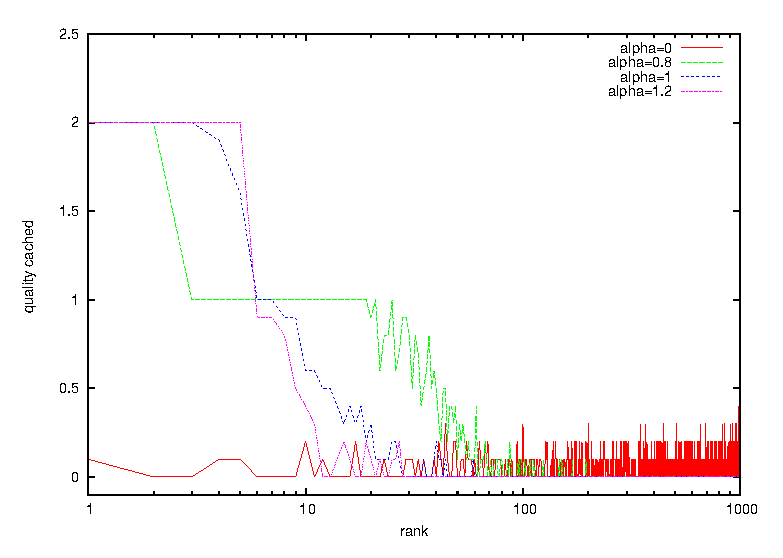
\includegraphics[angle=-90,width=\textwidth]{{eps/quality_cached}}
		\figLC{comparison}{Quality levels stored by the cache. Objects are ordered, in the x axis, from the most popular to the least. For each object, the cached quality is represented by a square of proportional size.
Observe that DedicatedCache and ProportionalDedicatedCache are the ones that best approximate RepresentationAware. This explains why the performance shown in the previous figure are similar. Observe that AllQualityLevels can story only few objects, due to the constraint to store all the quality levels for each one.
\AAra{Represent the \emph{representation utilization}, i.e. the utility provided by the fraction of requests that are matched by that copy. I expect that AllQualityLevels has a very low utilization since it stores an object representation even if it is never used. On the contrary, I expect that the representation utilization of RepresentationAware is the maximum. This is the REAL reason of our good performances. We store only the levels that is worth storing, contrarily to what ordinary CDNs seem to do.}
\AAra{power4 scale is used).}} 
	\end{figure*}


We make the load vary. \figR{comparison} shows that our Representation Aware strategy improves the average utility.

\subsection{The interdependence between link and cache capacity}
	\begin{figure}[t]
		\centering
		\includegraphics[width=0.25\textwidth]{{eps/capacity_impact_scenario}}
		\figLC{capacity_impact_scenario}{Incoming and outgoing link.} 
	\end{figure}

	\begin{figure}[t]
		\centering
		\includegraphics[angle=-90,width=0.50\textwidth]{{eps/capacity_vs_cache_impact}}
		\figLC{capacity_vs_cache_impact}{Impact of cache and bandwidth ratio between incoming and outgoing link. Utility is represented as the size of a black circle. Maximum utility, i.e. 1, is represented by the size of the white background circle.} 
	\end{figure}

	\begin{figure}[t]
		\centering
		\includegraphics[angle=-90,width=0.50\textwidth]{{eps/capacity_impact}}
		\figLC{capacity_impact}{Impact of input and output link capacity. We represent the breakdown of the cache content as a pie chart, each slice representing the number of videos stored at a certain quality level. Darker colors denote higher levels.} 
	\end{figure}
The optimal object and level selection heavily depends on three interdependent factors: the bandwidth available to retrieve objects (that we call \emph{incoming bandwidth}) and the bandwidth available to provide the cached content (that we call \emph{outgoing bandwidth}) and the cache space.
To investigate how the behavior of our optimal cache adapts to them, we consider, as in \figR{capacity_impact_scenario}, one node connected to a repository through an incoming link and to users through an outgoing link, whose capacities are $b_{in}$ and $b_{out}$, respectively. The node has a cache storage of capacity $S$. 

First, we observe that the benefits of caching inherently depend on the ratio between the incoming and outgoing link. In some case, the effect of caching is completely neutralized. Therefore a careless network planning which would not take into account this cases would imply a waste of resources.
	\begin{proposition}
	\propL{worthless}
	If $b_{out}\le b_{in}$ the cache is worthless.
	\end{proposition}
	\begin{IEEEproof}
	To prove this, we will find an upper bound of the achievable utility and we will show that it can be attained with no cache.
	The utility \eqR{objectiveFunction} depends on $n_v^{o,q}, \forall (o,q)\in O\times Q$, i.e. the number of request for the object $o$ we decide to serve at quality $q$.
	To find the upper bound, we suppose no limitation on the incoming link ($b_{in}=\infty$) and on the cache space $C=\infty$, such that it is possible to cache the entire catalog at the highest quality level. Therefore, the only constraint to take into account is that the traffic generated on the outgoing link must not exceed $b_{out}$. Suppose that ${\bar n}_v^{o,q}$ are the values that maximize the utility of this relaxed problem and that $\bar u$ is the utility provided to users by serving objects according to ${\bar n}_v^{o,q}$. Let us denote with $\bar y$ the bandwidth of the traffic generated on the outgoing link to provide the objects accordingly. Let us suppose to have no cache $C=0$. It is possible, even in this case, to provide the utility $\bar u$, by retrieving each requested object directly from the incoming link. This is possible because $\bar y \le b_{out} \le b_{in}$.
	\end{IEEEproof}

In other words, caching is beneficial only if the incoming bandwidth is larger than the outgoing. The smaller is the ratio between the two, the more caching can contribute to the user perception improvement. Otherwise stated, caching is really needed when the incoming bandwidth does not permit to retrieve all the objects at a rate that could follow the outgoing link capacity. It is worth stressing that, as we are concerned on user experience only, caching is worthless in every case it does not increase the utility. Obviously, even on those cases, caching has other benefits (as reducing the utilization of links), but they are mostly network-centric and will not be taken into account in this work, since we claim that, at the end, user satisfaction is the most important factor to consider.

Numerical results of \figR{capacity_vs_cache_impact} confirm what already stated. When The incoming bandwidth is much smaller that the outgoing (1/8, for instance), adding cache significantly boost user perceived performance. While incoming link becomes larger, the impact of caching is less important and becomes completely null (confirming \propR{worthless}) when the two links have the same capacity.

We now investigate which are the quality levels that is optimal to cache. We will find that it depends in particular on the outgoing bandwidth. Results are plotted in \figR{capacity_impact}.
We make the capacity of the two links vary and express it as a multiple of a default bandwidth value (490Kbps). We fix the catalog size at 10K objects and the cache to catalog size to 1/100. Due to \propR{worthless}, we represent only the cases in which the outgoing link is bigger than the incoming. Observe that, when the outgoing link is limited, only low quality levels are cached, regardless of the incoming link. This is expected: \emph{it is not worth caching high quality videos if not enough bandwidth is available to provide them}. Increasing the outgoing bandwidth makes storing higher quality videos beneficial.



\subsection{Collaboration}
	\begin{figure}[t]
		\centering
		\includegraphics[width=0.20\textwidth]{{eps/triangle}}
		\figLC{triangle}{Two peers connected by a peering link.} 
	\end{figure}

	\begin{figure}[t]
		\centering
		\includegraphics[angle=-90,width=0.50\textwidth]{{eps/intersection}}
		\figLC{intersection}{Benefits of collaboration. \AAra{Linear scale is used. Repeat it with powr4 scale} } 
	\end{figure}

\AAra{Collaboration can be twofold: by sharing the band or by sharing the cache space. I can make my peer use my band but avoiding him to use the objects in my cache, this means I'm sharing band but not cache.}
We now consider the topology of Fig.\AAra{Add it}, where a left AS and a right AS are connected to the content repository. A peering link is also established between the two ASes, through which they can collaborate, i.e. an AS can retrieve contents from the cache of the other, without using its private link to the repository. We make the capacity of peering link vary. When it is 0, the two ASes work in isolation, while increasing it fosters collaboration. When the peering link capacity is small, collaboration is limited, because this link cannot sustain all the traffic needed to download the contents from the sibling AS. 
The effect of collaboration is depicted in \figR{intersection}. We generate requests according to the Zipf distribution and we uniformly distribute them across the two ASes, so that, for each object, a certain ratio of the requests go to the left AS and the remaining part to the right AS.
The peering link capacity is expressed as a multiple of the default link capacity (490Mbps). The curve indicates the gain achieved by collaboration, i.e. how much the utility improves with respect to the case where no peering link is established. As expected, increasing the peering link capacity improves the utility perceived by users, but with a diminishing return. To explain this slope, we represent in the same plot the cache content of the two ASes. For each value of peering link capacity in the $\vec x$ axis, we represent the top 20 popular objects with a couple of grey squares. The size of the square on the left is proportional to the ratio of requests for that object received by the left AS, while the size of the right square is relative to the right AS. We place a ``x'' if the object is cached by the AS, while we left the square empty if the objects is not cached. Objects are ordered from the most popular (at the top) to the least.
The plot provides a fine-grained view of the caching strategy. Observe that, as expected, each AS tends to store the object if i) the object is popular, ii) the relative request ratio going to it is sufficiently large. For example, the left AS always prefers to store the 6th object instead of the 5th, despite of the smaller popularity, since it receives only a small ratio of request for that object (small square size).
We plot the ``x'' in darker color when both AS cache the same object. Observe that when peering link capacity is 0, the overlap between the two AS caches is large. This is an effect of the isolation. The overlap decreases while increasing the peering link capacity, since, if a certain object is stored by the right AS, for example, the left AS can retrieve it from there and, therefore, it does not need to store it in its cache and can use the saved space to store other objects. In other words, the two ASes collaborate by sharing their cache space. Sharing is bounded by the link capacity: the larger it is, the more the ASes can share their cache contents that, as a consequence, become more disjoint.

In the considered scenario, when peering link is equal to the default value (value on the $\vec x$ axis equal to 1), the sharing is complete, i.e. the cache contents are completely disjoint. Starting from this point, the utility improvement due to cache sharing no more holds if increasing the peering link capacity. Still, we observe a marginal improvement after $x=1$ value, which is due to a better utilization of the AS-to-repository links. Let us consider, for instance, the private link between the left AS and the repository. When no peering link is set up, the private link is used in order to maximize the utility of users of the left AS only, that roughly represent only half of the overall population, thus roughly contributing to only half of the global utility. On the contrary, when a peering link with enough capacity is established, the private link utilization is optimized taking into consideration the whole population of users, not only the half AS one. This permits to more effectively increase the global utilization and explains why utilization gain still improves even increasing the peering link capacity after the threshold of complete cache sharing.

\subsection{Realistic topologies}
\AAra{Should I differentiate link capacities based on the type of node? For example using 40Gbps link between tier I ASes \footnote{\url{http://en.wikipedia.org/wiki/Core_router#History} } }
We consider now the impact of caching on a multi-AS environment. Caching is nowadays operated on tier III networks (that we will interchangeably access networks), by means of CDN or HTTP proxies. As already observed by \cite{Agyapong2012}, tier II and I operators lack incentives in caching and will do it only if adequately rewarded by an explicit economic exchange. In this section we show that caching everywhere (in all the Internet tiers) is beneficial for users. Therefore, it is worth rewarding higher tier operators to convince them to cache.

We generate a network of 100 nodes in accordance to the Barabasi-Albert model, which is considered to approximate the properties of the AS-level Internet graph.
% "In inter-AS type topologies (i.e., similar to BA)"
We consider the 50 nodes with the smallest degree as the access networks. We connect the clients and the content repositories to these nodes. We uniformly distribute the requests and the object among these nodes.







%%%%%%%%%%%%%%%%%%%%%%%%%%%%%%%%%%%%%%%%%%%%%%%%%%%%%
%%%%%%%% Discussion %%%%%%%%%%%%%%%%%%%%%%%%%%%%%%%%%
%%%%%%%%%%%%%%%%%%%%%%%%%%%%%%%%%%%%%%%%%%%%%%%%%%%%%
\section{Discussion}
The model we wrote assigns to each user a data-rate value for each download, that can be thought as computed by a central brain of the system. While this assumption provides us the theoretical optimal working point of the entire system, it does not match the way video streaming is done today
. Indeed, in current video streaming protocols the client adjusts the download rate based on the available bandwidth estimation. In current client-driven video streaming the issue described by\cite{Lee2014} may happen: suppose a cache is storing a video at quality $q=3$ and a client is retrieving it from there; if the bandwidth between the client and the cache is large, a client would request a video at higher quality, say $q=4$, which may not be stored in the same cache and must be retrieved by some other source; the bandwidth between the client and this other source may be smaller, thus not supporting the delivery of $q=4$. To overcome this issue we assume to implement some control logic also in the sender, i.e. cache server or permanent server, implementing a shaping mechanism to react to client requests with a timing such to force client to download video at the cached quality level. This is a reasonable assumption given that sender-driven rate adaptation mechanisms have been widely studied in the literature. We also assume that the representation selection is not operated based only on the estimates collected by the client, but is guided by a ``control plane'' that has the global vision of the network and can make optimal choices, as envisioned by ~\cite{Liu2012a}.


From a conceptual viewpoint, the problem that our model aims to solve can be formulated as follows: we have facilities, i.e. link capacities and caches, which are at our disposal and are empty at the initial instant $0$. We have to match a set of user requests for videos. Each video is 5 min long, What is the best facility allocation during the interval $[0,5 min]$ in order to have the best user utility? Since we suppose that all videos start and end at the same instant, what we observe at any instant is exactly the same. In other words we can adopt a snapshot approach, as done in optimization works~\cite{Toni2014,Zhang2013}, i.e. we do not need to look into the dynamics of the system. A more realistic model should account for different starting and ending times for different objects, in order to exploit, for example, the free bandwidth left by a flow that ended.

Moreover, we do not take into account the dynamics of the network, which can have a relevant impact. For example, if a new user joins the network, she has to be assigned some bandwidth, thus potentially implying the reduction of data-rate assigned to the previous users with consequent quality level fluctuations. As other optimization based work on video streaming~\cite{Toni2014}, we do not take into account these fluctuations. These considerations are out of our scope and are barely treatable with an optimization approach like ours. We plan to separately consider them in a future work, where we will propose control algorithms that can make the network approximately converge to the solution given by our current model and we will evaluate them by means of simulation.

Observe that this model (see \eqR{multiple_src}) admits the possibility that a user downloads a video from different sources in parallel, as in \cite{Liu2012b} \AAra{Controlla se davvero la citazione dice questo}. We compute the download rate as the sum of the download rate from each source. This is possible when a client issue different HTTP GET with consecutive byte ranges, which will be retrieved in parallel.

Contrarily to \cite{Toni2014} and others, we consider only one type of network, namely ADSL, and we do not distinguish video categories (sport, movie, documentary, ... ).




% ==============================================================================
% Conclusion
% ==============================================================================

\section{Conclusions}
\secL{conclusion}



 
\section*{Acknowledgment}
\noindent  

\begin{small}
\bibliographystyle{abbrv}
\bibliography{library} % I DON'T WANT MENDELEY EXPORT UNTIL IT IS FULL OF RUBBISH! WE MAY ALSO HAVE DUP ITEMS!
\end{small}
% drossi@pink:~/paper/drafts/costaware-icn14$ wc *bib
%    15   219  1975 dario.bib
%  1542  8506 72928 library.bib
%    77   320  2731 referencesICN.bib

%\include{examples}
%\include{appendix}
\end{document}


